\begin{surferPage}[Kummer-Quartic]{משטח ממעלה רביעית של קומר}
    בשנת 1875, היה אדוארד קומֶר
    \textenglish{(Eduard Kummer)}
      האדם הראשון שניסח בצורה מפורשת את השאלה
    בדב המספר המרבי $\mu(d)$ של נקודות סינגולריות במשטח ממעלה
    $d$, 
    וזאת כאשר חקר את המקרה של משטחים ממעלה רביעית (המכונים \emph{quartics}). 
  
  הוא הראה ש-$\mu(4)=16$. לאחר מכן, הוא חקר לעומק משטחים ממעלה רביעית בעלי $16$
    נקודות סינגולריות.
    המשוואה הבאה יוצרת משפחה של משטחים בעלי מאפיינים יפים במיוחד:
    \[\bigl(x^2+y^2+z^2-\mu^2\bigr)^2 - \lambda
    \,y_0\,y_1\,y_2\,y_3,\]
    כאשר $\mu$ הוא פרמטר חופשי, ואילו 
    $\lambda = \frac{3\mu^2-1}{3-\mu^2}$; המשתנים $y_i$ מסמלים את הצלעות של
    ארבעון (פירמידה משולשת) משוכלל {\small
    $y_0=1-z-\sqrt{2}x$, \  
    $y_1=1-z+\sqrt{2}x$, \ 
    $y_2=1+z+\sqrt{2}y$, \ 
    $y_3=1+z-\sqrt{2}y$}
  על-מנת שהמשטח יהיה סימטרי.
  לא כל המשטחים החברים במשפחה זה כוללים בדיוק $16$ נקודות סינגולריות.
  אם כי הדבר נכון לגבי רובם:
  \begin{center}
    \vspace*{-0.2cm}\hspace*{-0.2cm}
    \begin{tabular}{@{}c@{\,}c@{\,}c@{\,}c@{\,}c@{}}
      \begin{tabular}{@{}c@{}}
        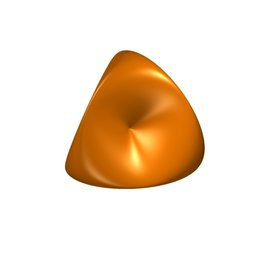
\includegraphics[height=1.4cm]{./../../common/images/kummer_0}
      \end{tabular}
      &
      \begin{tabular}{@{}c@{}}
        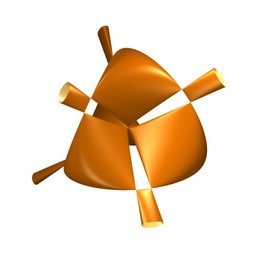
\includegraphics[height=1.4cm]{./../../common/images/kummer_1}
      \end{tabular}
      &
      \begin{tabular}{@{}c@{}}
        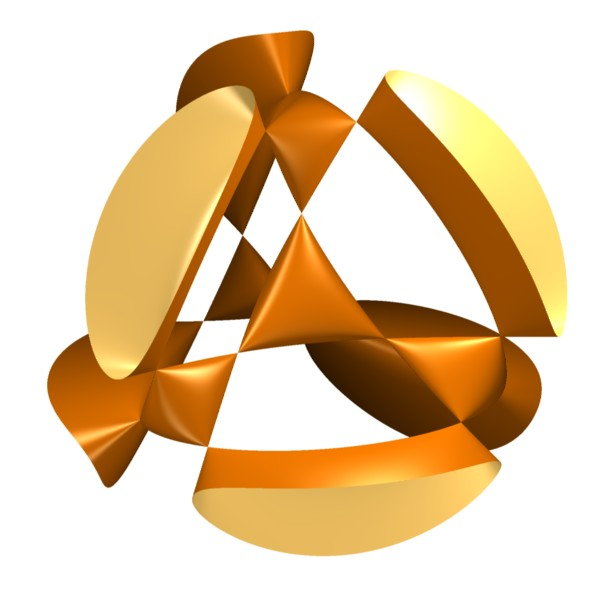
\includegraphics[height=1.4cm]{./../../common/images/kummer_2}
      \end{tabular}
      &
      \begin{tabular}{@{}c@{}}
        
\includegraphics[height=1.4cm]{./../../common/images/kummer_3}
      \end{tabular}
    \end{tabular}
  \end{center}
  \vspace{-0,2cm}  
   עבור ערכים מסוימים של הפרמטרים, חלק מנקודות הסינגולריות עשויות
  לחפוף זו לזו.
\end{surferPage}
